\section{Undirected log-linear models}
\label{sec:undirected}

% DONE: need more of a transition from previous sections
Recall that we used tensor factorization and composite likelihood
to estimate the hidden marginals $Z_\sC = \BP(\vh_\sC)$ and $\mOpp{v}{i} = \BP(x_v \mid h_i)$.
For directed models, obtaining the local conditional tables from $Z_\sC$ simply requires
renormalizing $Z_\sC$.
For undirected log-linear models, the canonical parameters cannot be obtained
locally.
Fortunately, we can construct a convex optimization problem
by relating the recovered conditional moments with the expected features of
the log-linear model.

% Define model
As before, let $\sG$ be a graphical model with observed variables $\bx$ and hidden variables $\bh$
(see \figureref{examples-mrf} for an example).
For each clique $\sC \in \sG$, we have a feature vector $\phi_\sC(\vx_\sC, \vh_\sC)$,
where $\vx_\sC$ and $\vh_\sC$ are the observed and hidden variables in $\sC$, respectively.
Let $\phi(\vx, \vh) = \sum_{\sC \in \sG} \theta^\top \phi_\sC(\vx_\sC,\vh_\sC)$ be the global feature vector.
We consider log-linear models of the following form:
\begin{align*}
p_\theta(\vx, \vh) &= \exp\left( \theta^\top \phi(\vx,\vh) - A(\theta) \right),
\end{align*}
where $A(\theta) = \log \sum_{\vx, \vh}  \exp( \theta^\top \phi(\vx,\vh) )$ is the log-partition function.

% FIGURE: example
\begin{figure}
  \centering
  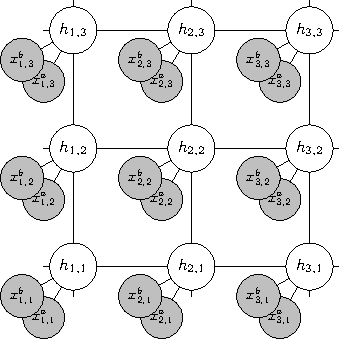
\includegraphics[width=0.6\columnwidth]{figures/mrf.pdf}
%  \subimport{figures/}{mrf.tikz}
  \caption{Example: undirected grid model where each hidden variable has two
  conditionally independent observations.
  We derive a consistent estimate.}
  \label{fig:examples-mrf}
\end{figure}

%As an example, consider an undirected grid model in \figureref{examples-mrf},
%where each hidden variable has two conditionally independent observations.
%In practice, if two features are known to be independent, then they can
  %be separated into independent observed variables.
%Let the parameters of the model be $O \eqdef \Phi(x^a_{i,j}, h_{i,j})
  %= \Phi(x^b_{i,j}, h_{i,j})$ and $T \eqdef \Phi(h_{i,j}, h_{i \pm 1,j \pm 1})$. 
%Note that as this is an undirected model, the clique marginals do not
  %correspond to the parameters of the model.
%To recover the parameters of this model, note that every hidden
%  variable, $h_{ij} \in \sH$ is a bottleneck, with views
%  $x^{a}_{ij},x^{b}_{ij}$ and any other observed variable in the graph. 
%Thus, \LearnMarginals will be able to learn the marginals of each clique
%  and \LearnLogLinear will give us a consistent estimate of the
%  parameters. 

Of course, the log-likelihood is non-concave:
\begin{align*}
  L_\text{unsup}(\theta) \eqdef \E_{\vx \sim p^*}[\log \sum_{\vh \in \sH} p_\theta(\vx,\vh)],
\end{align*}
where we are assuming for simplicity that we have infinite data drawn from the true distribution $p^*$.
% PL: this doesn't make sense
%While $\phi_\sC(x,h)$ can be an arbitrary featurization, we assume
%  without loss of generality that $\phi_\sC(x,h)$ are the indicator
%  features $\BI[x,h]$\footnote{Note that $\BI[x,h]$ are sufficient
%  statistics for the model, and hence we do not lose any statistical
%  efficiency in using them.}.

%In this section, we will show that we can extend the results to
  %undirected graphical models parameterized as log-linear latent variable
  %models.
On the other hand, 
if we were able to observe $\vh$, we would optimize the \emph{supervised} likelihood, which is concave:
\begin{align}
L_\text{sup}(\theta) &\eqdef \E_{(\vx,\vh) \sim p^*}[\log p_\theta(\vx,\vh)] \nonumber \\
                     &= \theta^\top \left(\sum_{\sC \in \sG} \E[\phi(\vx_\sC,\vh_\sC)]\right) - A(\theta).
\label{eqn:logLinearSupervised}
\end{align}
While we don't have supervised data,
recall that the method of moments provides the hidden marginals $Z_\sC = \BP(\vh_\sC)$
and conditional moments $\mOpp{v}{i} = \Pr(x_v \mid h_i)$.
Assuming our graphical model is in canonical form (\lemmaref{reduction}),
every observed variable is connected to exactly one hidden variable.
Then $Z_\sC$ and $\mOpp{v}{i}$ directly yield marginals for every clique $\BP(\vx_\sC, \vh_\sC)$.
Given these marginals, we can compute the expected local feature vector:
\begin{align}
\label{eqn:logLinearFeatures}
\mu_\sC \eqdef \E[\phi(\vx_\sC,\vh_\sC)] = \sum_{\vx_\sC,\vh_\sC} \BP(\vx_\sC,\vh_\sC) \phi(\vx_\sC,\vh_\sC).
\end{align}
Note that $\{\mu_\sC\}_{\sC \in \sG}$ are exactly the sufficient statistics of the model (\equationref{logLinearSupervised}),
so we can optimize the supervised likelihood objective without actually having any supervised data!
In the finite data regime, the method of moments yields the estimate
$\hat \mu^\text{mom}_\sC$ which approximates the true $\mu_\sC$.
In supervised learning, we obtain a different estimate $\hat\mu^\text{sup}_\sC$ of $\mu_\sC$ based on an empirical average
over data points.
In the limit of infinite data, both estimators converge to $\mu_\sC$.

%We exploit the connection between the moments of the clique potentials and
  %the log-partition function to show that learning parameters is convex
  %given the clique marginals $Z_\sC$. 
%The end result is a consistent estimator for log-linear
  %latent-variable models which satisfy \propertyref{exclusive-views}.
%Finally, we generalize the result to classes when only a subset of the
  %clique marginals can be learned.

%As before, our objective is to find a set of parameters $\hat \theta$
%  that maximize the likelihood of data $\sD$.
%\begin{align}
%  \hat \theta 
%      &= \arg\max_{\theta} \sum_{\vx \in \sD} \log p_\theta(\vx) \nonumber \\
%      &= \arg\max_{\theta} \sum_{\vx \in \sD} \log \sum_{\vh \in \sH} p_\theta(\vx,\vh) \nonumber \\
%      &= \arg\max_{\theta} \sum_{\vx \in \sD} \log \sum_{\vh \in \sH} \exp( \theta^\top\phi(\vx,\vh) - A(\theta) ). \label{eqn:obj-ml}
%\end{align}
%Note that this problem is not concave in $\theta$. 
%
%\note{Consider the supervised setting.
%As we get infinite amounts of data, we get this simple form.
%As MoM is a consistent estimator for marginals, we can optimize this
%  likelihood and it is consistent.
%}

%However, given the moments $\E[ \phi_\sC(\vx,\vh) ] = Z_\sC$, the
%  problem simplifies to,
%\begin{align}
%  \hat \theta 
%  &= \arg\max_{\theta} \sum_{\sC \in \sG} \theta_\sC^\top Z_\sC - A(\theta), \label{eqn:obj}
%\end{align}
%which is concave in $\theta$.
\algorithmref{undirected} summarizes our approach.
In \sectionref{exclusiveViews}, we showed that $\LearnMarginals$ is a consistent
estimator for $Z_\sC$ for any bottlenecked clique in the graphical model. 
Consequently, \algorithmref{undirected}
is also a consistent estimator.\footnote{Of course, the log-linear model must be identifiable.
Identifability is violated, for example, if two components of $\phi(\vx_\sC, \vh_\sC)$ were identical.
In general, we can identify the parameters up to the kernel of $\nabla^2 A(\theta)$.}

\renewcommand{\algorithmicrequire}{\textbf{Input:}}
\renewcommand{\algorithmicensure}{\textbf{Output:}}
\begin{algorithm}
  \caption{\LearnParameters (for undirected models)}
  \label{algo:undirected}
  \begin{algorithmic}
    \REQUIRE Conditional moments $\mOpp{v}{i}$ and clique marginals $Z_\sC$.
    \ENSURE Parameters $\theta$
      \STATE Compute expected features $\{\mu_\sC\}_{\sC \in \sG}$ (\equationref{logLinearFeatures}).
      \STATE Optimize \equationref{logLinearSupervised}.
    \end{algorithmic}
\end{algorithm}

\subsection{Pseudolikelihood}
\label{sec:pseudolikelihood}

Unlike for directed models, in the undirected case,
graphs with high treewidth present a challenge
for even fully-supervised maximum likelihood due to the intractability of the log-partition function $A(\theta)$.
%One can employ various variational approximations of $A(\theta)$ \cite{wainwright08varinf},
This motivates looking at pseudolikelihood objective of \citep{besag75pseudo} for a computationally more
efficient solution.
The pseudolikelihood objective is a sum over the log-probability of each variable $a$ given its neighbors $\sN(a)$:
\begin{align}
  \label{eqn:pseudolikelihood}
L_\text{pseudo}(\theta) \eqdef \E_{(\bx,\bh) \sim p^*}\left[\sum_{a \in X \cup H} \log p_\theta(a \mid \sN(a))\right].
\end{align}
In the fully-supervised setting, it is well-known that pseudolikelihood provides computationally efficient consistent estimates,
albeit at the cost of statistical efficiency.
Coincidentally, this is the same high-level motivation for using method of moments in the first place.

Let $\phi_{a,\sN(a)}(a, \sN(a)) = \sum_{\sC \ni a} \phi_\sC(\bx_\sC,\bh_\sC)$
denote the sum over cliques $\sC$ that contain $a$; note that $\phi_{a, \sN(a)}$ only depends on $a$ and its neighbors $\sN(a)$.
We can write each conditional log-likelihood as:
\begin{align*}
p_\theta(a \mid \sN(a)) = \exp(\theta^\top\phi_{a,\sN(a)}(a, \sN(a)) - A_a(\theta; \sN(a))),
\end{align*}
where the conditional log-partition function $A_a(\theta; \sN(a)) = \log \sum_{a'} \exp(\theta^\top\phi_{a,\sN(a)}(a', \sN(a)))$
involves marginalizing only over a single variable.

If we knew $\mu_{a,\sN(a)} \eqdef \E[\phi_{a,\sN(a)}(a,\sN(a))]$,
then we would be able to optimize the pseudolikelihood objective again without
having access to any labeled data.
%The pseudolikelihood also replaces the log-partition function
%  $A(\theta)$ with a sum over the variables in the neighborhood:
%  $A_a(\theta; x_{\sN(a)}) = \sum_{a' \in \{a\} \union \sN(a)}
%  \exp(\theta^\top\phi_{\sN(a)}(a'))$.
Note that $\{a\}\cup\sN(a)$ in general does not form a clique.
Fortunately, \lemmaref{bottleneck-views} holds for all biconnected subgraphs.
We can break $\{a\}\cup\sN(a)$ into a collection of biconnected subgraphs 
  % PL: this is not necessary
  %thus the uniformly bottlenecked assumption alone is not sufficient to
  %guarantee exclusive views for each variable in that subgraph.
%However, when we do have exclusive views for each neighborhood, as in
 (e.g. \figureref{examples-mrf}).
  Therefore, we can adapt our algorithm ($\LearnMarginals$) to estimate all marginals of the form $Z_{a,\sN(a)} \eqdef \Pr(a,\sN(a))$,
  from which we can compute the features $\mu_{a,\sN(a)}$,
  and optimize \equationref{pseudolikelihood} to obtain a consistent estimate of $\theta$.

% Arun: WRONG
% The pseudolikelihood also replaces the log-partition function $A(\theta)$
% with a sum over the variables in the neighborhood: $A_a(\theta; x_{\sN(a)}) = \sum_{a' \in \{a\} \union \sN(a)} \exp(\theta^\top\phi_{\sN(a)}(a'))$,
% which cannot be computed from just the hidden clique marginals $Z_\sC$,
% since the neighbors $\sN(a)$ in general do not form a clique.
% We adapt our earlier algorithm ($\LearnClique$) to estimate the
%   marginals over all neighborhoods $Z_{\sN(a)}$ by noting that
%   \lemmaref{bottleneck-views} guarantees exclusive views for any connected
%   subgraph of $\sG$, not just cliques.

While this method is only viable for graphs of low degree, i.e.\@ when $|\sN(a)|$ is small,
it can handle graphs with high treewidth.
For example, in the grid model, the degree is only 4.
Note that neither sample nor computational complexity depends on the treewidth.

\paragraph{Learning with partial moment constraints.}

In general, it might be case that we only have exclusive views for a subset of the cliques.
In this case, we can estimate the expected features $\mu_\sC$ for those cliques
  and use posterior regularization \citep{graca08em} or the generalized expectation criteria \citep{mann08ge}
  to encourage $\E_{p_\theta}[\phi(\vx_\sC,\vh_\sC)]$ to match $\mu_\sC$.
The resulting objective functions are still non-convex, but we expect
  local optima to be alleviated. 

%but in practice we observed that the extra information $\mu_\sC$ helps alleviate local optima.
%We can then integrate these constraints using posterior regularization \citep{graca08em}:
%\begin{align}
%L_\text{pr}(\theta) \eqdef L_\text{unsup}(\theta) + C\min_{q \in \sQ} \text{KL}(q(\vx,\vh) \| p_\theta(\vx,\vh)).
%\end{align}
%The main idea is to regularize the parameters towards values that produce the 
%While the optimization problem \eqref{eqn:obj-ml} is non-convex, we
  %expect that the measurements aid recover of parameters, and indeed see
  %this is true for experiments on simulated data.
%\todo{Include figure}

%Posterior regularization optimizes the following objective,
%\begin{align*}
%  \hat \theta &= \arg\min_{\theta} \arg\min_{q \in \sQ} \KL( q(\vx,\vh) \| p_{\theta}(\vx, \vh) ),
%\end{align*}
%where $q$ is a marginal distribution that belongs in constrained set
%$\sQ$. In our case, $\sQ$ is constrained to agree with the partial
%moments we recovered using \LearnMarginals, i.e. 
%\begin{align*}
%  \sQ &= \{ q(\vx,\vh) \given \forall \sC \in \sP ~ \E_{q(\vx,\vh)}[\phi_\sC(\vx, \vh)] = Z_\sC \}.
%\end{align*}

%In practice, we would like to regularize for error in our
%  estimates of $Z_\sC$; to do so, we use the measurements model of
%  \citet{liang09measurements} which defines a Bayesian model for the noise
%  in the marginals $Z_\sC$. The resultant optimization problem is,
%\begin{align*}
%  \hat\theta 
%  &= \arg\min_\theta - \sum_{x \in \sD} \log p_\theta(x) + \half \eta_\theta \| \theta \|^2 \\
%  &\quad + \half \eta_\beta \| Z_\sC - \sum_{\vx \in \sD} \E_{\theta}[\phi_\sC(\vx,\vh)] \|^2,
%\end{align*}
%where $\eta_\theta$ and $\eta_\beta$ are regularization parameters. 

%
%However, the objective \equationref{obj} requires us to compute the
%  partition function, $A(\theta)$ and its gradient. 
%This scales with the treewidth of the model, which is the number
%  of rows/columns of the grid in this example, and hence can be
%  intractable.
%A more computationally efficient, but still consistent, alternative is
%to optimize the pseudo-likelihood \todo{how do I write this out}.


